\documentclass[aspectratio=169]{beamer}

\usepackage{amsmath}
\usepackage{tikz}
\usepackage{beamerpkg}

\title{beamerpkg demo}
\author{Demo}
\date{}

\begin{document}

\begin{frame}{Normal Beamer stays normal}
  \begin{columns}[T]
    \column{0.48\textwidth}
      \begin{block}{Equation}
      \[
        \frac{\partial c}{\partial t} = \nabla\!\cdot\!\left(M\nabla\mu\right)
      \]
      \end{block}
      \pause
      \begin{itemize}
        \item equations remain vector PDF;
        \item overlays remain Beamer pages;
        \item TikZ remains TikZ.
      \end{itemize}
    \column{0.48\textwidth}
      \begin{tikzpicture}[scale=0.8]
        \draw[->] (0,0) -- (4,0) node[right] {$x$};
        \draw[->] (0,0) -- (0,3) node[above] {$y$};
        \draw[thick] (0.3,0.4) .. controls (1.5,2.8) and (2.5,0.2) .. (3.7,2.4);
      \end{tikzpicture}
  \end{columns}
\end{frame}

\begin{frame}{Lightweight PDF page transition}
  \transfade[duration=0.25]
  \centering
  \Large
  This frame uses Beamer's standard PDF fade transition.

  \vspace{1em}
  \normalsize
  No video, JavaScript, or Acrobat-specific animation package is involved.
\end{frame}

\begin{frame}{Timed overlays as pseudo-animation}
  % Auto-advance the first three overlay pages; stop on the final state.
  \transduration<1-3>{0.55}
  \transduration<4>{}

  \centering
  \begin{tikzpicture}[x=1.35cm,y=1.35cm]
    \draw[->,thick] (0,0) -- (5.2,0) node[right] {$t$};
    \foreach \x in {0,1,2,3,4}
      \draw (\x,-0.08) -- (\x,0.08);

    \only<1>{\fill (0.5,0.7) circle (0.12);}
    \only<2>{\fill (1.5,0.7) circle (0.12);}
    \only<3>{\fill (2.5,0.7) circle (0.12);}
    \only<4>{\fill (3.5,0.7) circle (0.12);}

    \node[below] at (2.2,-0.35) {four ordinary Beamer overlay pages};
  \end{tikzpicture}

  \vspace{1em}
  The first three overlays advance automatically; the last one waits for input.
\end{frame}

\begin{frame}{Standard Beamer movie: wrapperless discovery}
  \begin{columns}
    \column{0.38\textwidth}
      This is a stock Beamer \texttt{\\movie}. The packer discovers the
      external MP4 directly from the PDF annotation. In pdfpc it is
      click-to-play.
    \column{0.58\textwidth}
      \movie[loop,showcontrols]
        {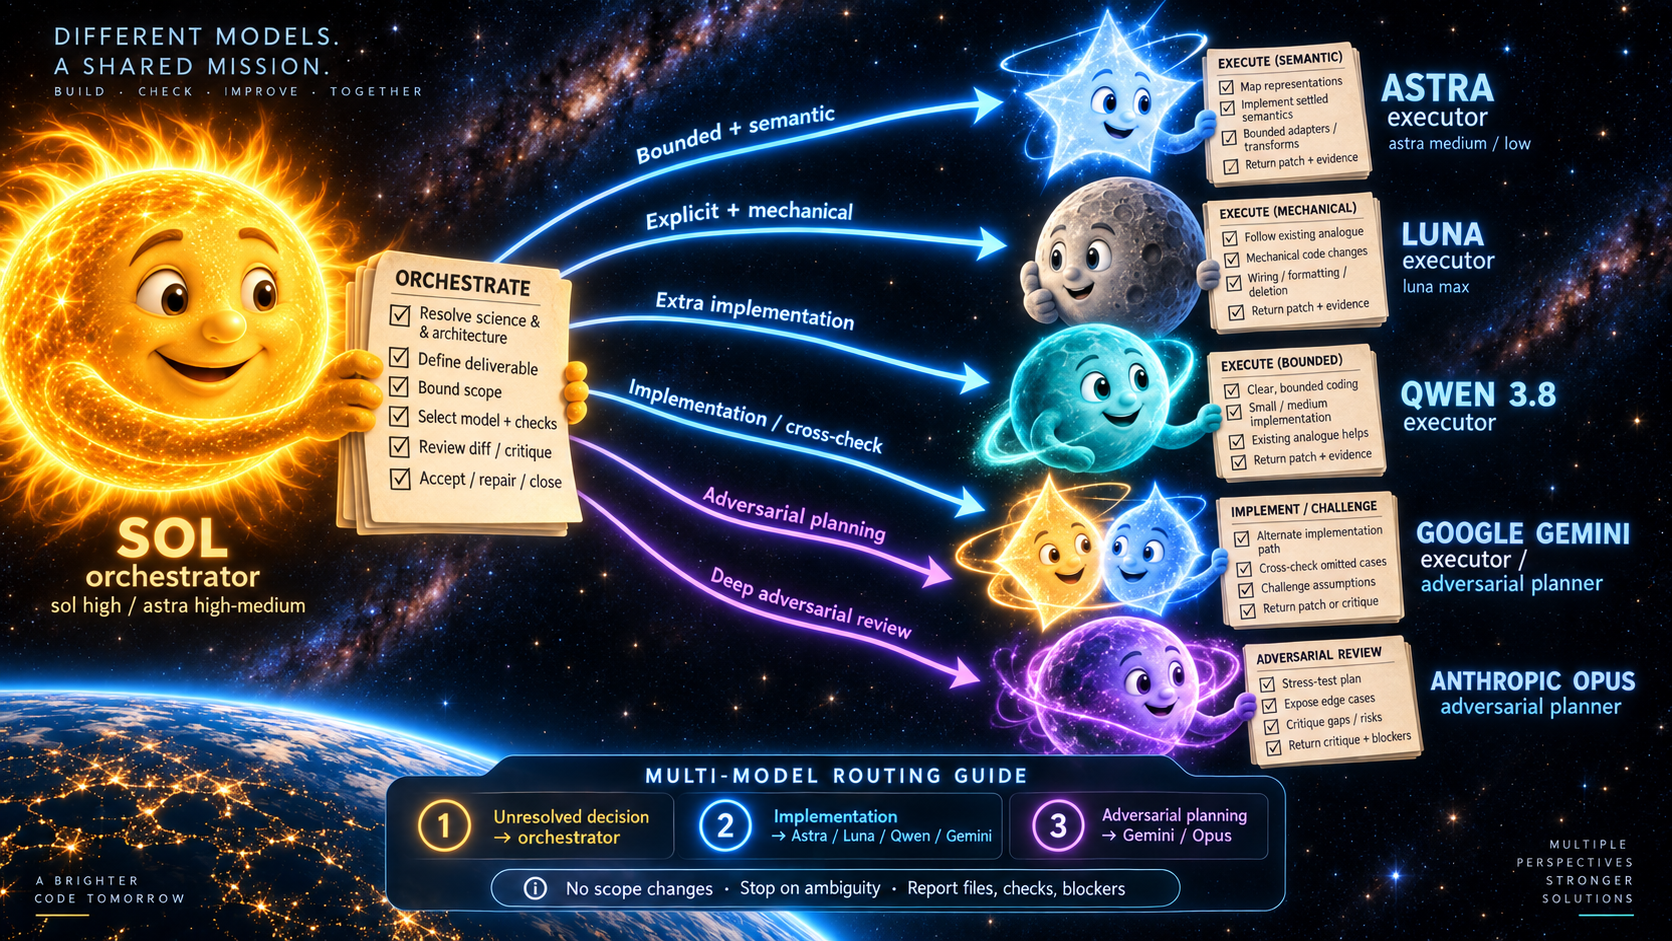
\includegraphics[width=\linewidth]{media/video-poster_big.png}}
        {media/gemini_generated_video_b2693757.mp4}
  \end{columns}
\end{frame}

\begin{frame}{Autoplay video (pdfpc-specific)}
  \begin{columns}
    \column{0.38\textwidth}
      The slide is still ordinary Beamer/PDF. The pdfpc-specific launch link
      starts the same packaged video automatically and loops it while the slide
      is shown.
    \column{0.58\textwidth}
      \pkgpdfpcmovie[autostart&loop]
        {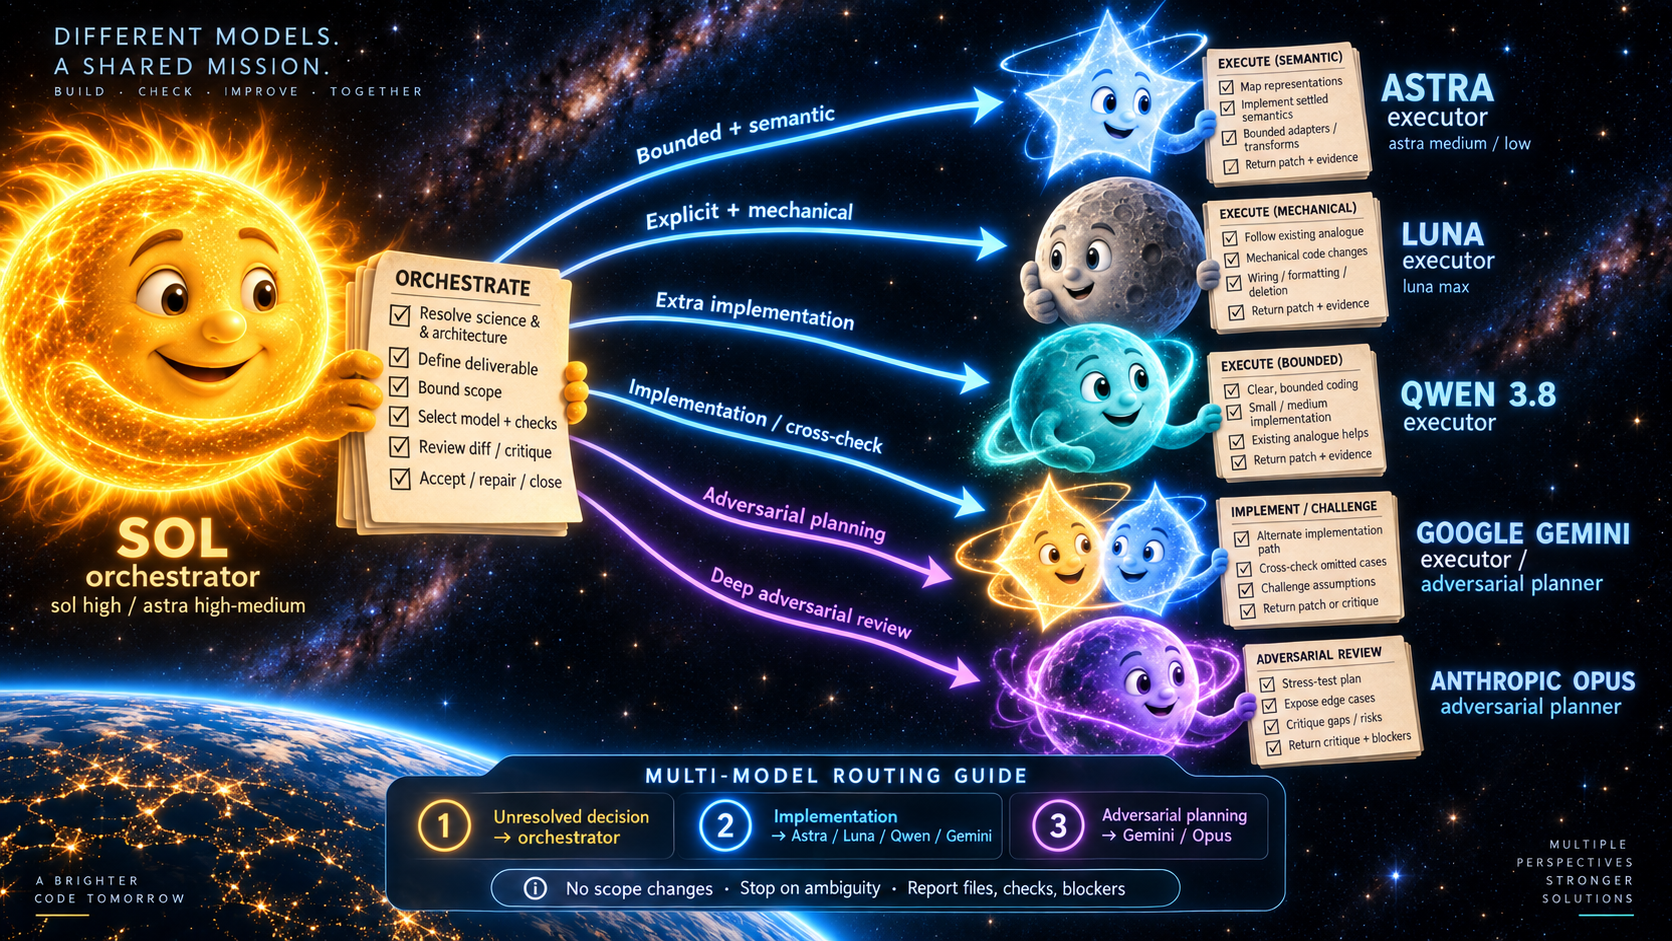
\includegraphics[width=\linewidth]{media/video-poster_big.png}}
        {media/gemini_generated_video_b2693757.mp4}
  \end{columns}
\end{frame}

\begin{frame}{Back to ordinary overlays}
  \centering
  \only<1>{Static PDF content.}
  \only<2>{No HTML renderer involved.}
  \only<3>{The media layer has not changed slide rendering.}
\end{frame}

\end{document}
